\section{Business Process Modeling Notation (BPMN)}

\subsection{�Que es?}

Al interior de una organizaci�n es importante documentar y especificar los diferentes procesos que se deben llevar a cabo. A menudo, se suelen utilizar diagramas de flujo o incluso descripciones textuales. Desafortunadamente, estas t�cnicas se quedan cortas a la hora de describir procesos mas complejos, y mas a�n cuando cada organizaci�n define su propia notaci�n, dificultando el entendimiento de los diferentes modelos que se realizan al interior de la organizaci�n. Es por esto que se hace necesario crear una notaci�n est�ndar y especifica para describir este tipo de procesos.

BPMN, Business Process Modeling Notation, es precisamente el est�ndar que se viene adoptando a nivel masivo para la creaci�n y descripci�n de los diferentes procesos que hacen parte del funcionamiento de las diferentes organizaciones.


Con el est�ndar BPMN, se tienen en cuenta diferentes elementos b�sicos que sirven como herramientas para crear y estructurar los diferentes modelos que se quieran hacer. Estos elementos solo describen una forma b�sica de uso, pues BPMN permite personalizar los elementos a utilizar, siempre y cuando los cambios realizados no dificulten el proceso de entendimiento de los modelos.

\subsection{Enlaces}

Los enlaces sirven para unir o bifurcar el flujo de secuencia de un modelo. Son utilizadas cuando es necesario tomar alg�n tipo de decisi�n que lleve a tomar uno o varios caminos alternos. Existen varios tipos de enlaces, como lo son los enlaces exclusivos (XOR), paralelos (AND), inclusivos (OR) y complejos. A continuaci�n, se muestran ejemplos de aplicaci�n de cada uno de estos enlaces.

\begin{figure}[!htb]
  \begin{center}
    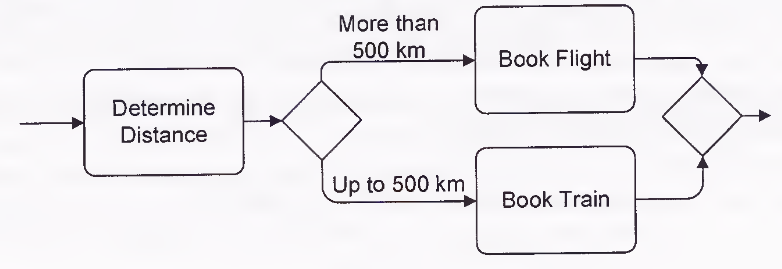
\includegraphics[width=11cm]{./imagenes/gateway_exclusivo.png}
    \caption{Ejemplo de uso del enlace exclusivo}
    \label{fig:gateway_exclusivo}
    \textbf{Fuente:}  \cite{bpmn2}
  \end{center}
\end{figure}

En este caso (Figura \ref{fig:gateway_exclusivo}), se realiza la actividad \textit{Determinar distancia} y se decide que tipo de medio de transporte se debe utilizar. N�tese que luego de realizar la reserva, se vuelve a unir el flujo de secuencia del modelo, ya que no se sabe en la pr�ctica cual de las 2 alternativas ser� la seleccionada.

\begin{figure}[!htb]
  \begin{center}
    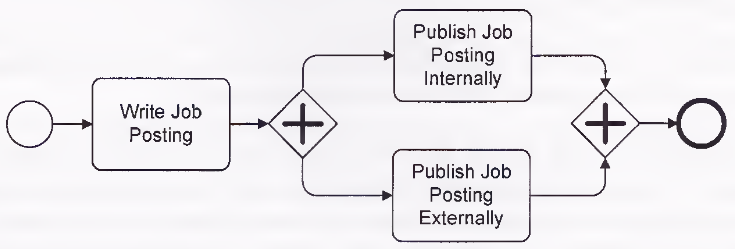
\includegraphics[width=11cm]{./imagenes/gateway_paralelo.png}
    \caption{Ejemplo de uso del enlace paralelo}
    \label{fig:gateway_paralelo}
    \textbf{Fuente:}  \cite{bpmn2}
  \end{center}
\end{figure}

En la figura \ref{fig:gateway_paralelo} se ve un ejemplo de uso de este enlace. Aqu�, luego de que se redacta la oferta de trabajo, le procede a publicarla, tanto interna como externamente. En este caso, se utiliza el enlace paralelo para agilizar el proceso de publicaci�n.

\begin{figure}[!htb]
  \begin{center}
    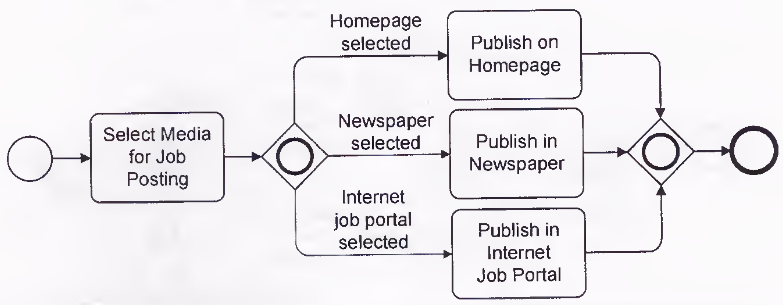
\includegraphics[width=11cm]{./imagenes/gateway_inclusivo.png}
    \caption{Ejemplo de uso del enlace inclusivo}
    \label{fig:gateway_inclusivo}
    \textbf{Fuente:}  \cite{bpmn2}
  \end{center}
\end{figure}


En la figura \ref{fig:gateway_inclusivo} se ve un ejemplo de uso en donde a partir de la actividad ``Seleccionar medio para publicar oferta de trabajo'' se pueden seleccionar una o varias opciones. Cualquier combinaci�n de opciones, que al menos contenga una opci�n, es v�lida.

\begin{figure}[!htb]
  \begin{center}
    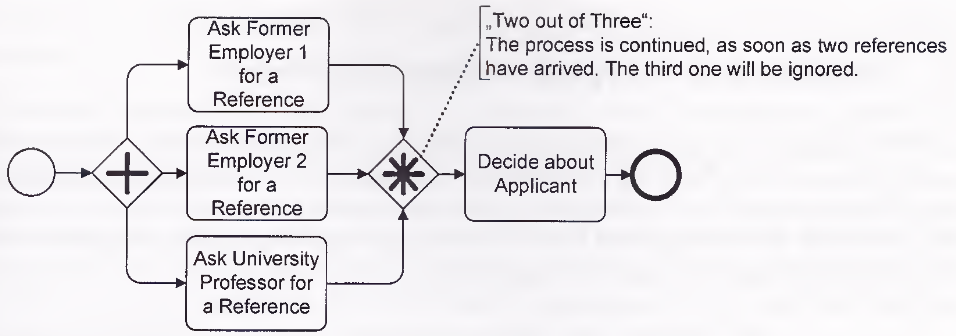
\includegraphics[width=11cm]{./imagenes/gateway_complejo.png}
    \caption{Ejemplo de uso del enlace complejo}
    \label{fig:gateway_complejo}
    \textbf{Fuente:}  \cite{bpmn2}
  \end{center}
\end{figure}


En el ejemplo mostrado en la figura \ref{fig:gateway_complejo}, se requiere la referencia de 2 empleadores previos y de la universidad. En realidad, solo son necesarias dos referencias, pero para estar seguros se piden tres, por lo que tan pronto como llegan las primeras 2 referencias, la tercera puede ser ignorada sin mayor problema.

\subsection{Colaboraci�n}

A menudo, en un proceso intervienen diferentes partes interesadas (\textbf{\textit{Stakeholders}}) y es necesario ver el proceso de manera global, de manera que el paso de mensajes entre las partes implicadas sea mas claro. A este tipo de diagramas se les llama \textbf{diagrama de colaboraci�n}

La figura \ref{fig:diagrama_colaboracion} muestra como es la interacci�n entre un aspirante y una empresa en el proceso de acceder a una oferta de empleo. Puede verse como, entre las actividades que ejecuta cada una de las partes, existe un paso de mensaje que une ambos procesos. Esta uni�n se representa por una flecha con linea punteada, donde un extremo tiene un circulo y el otro una flecha vac�a que indica la direcci�n del mensaje.

\begin{figure}[!htb]
  \begin{center}
    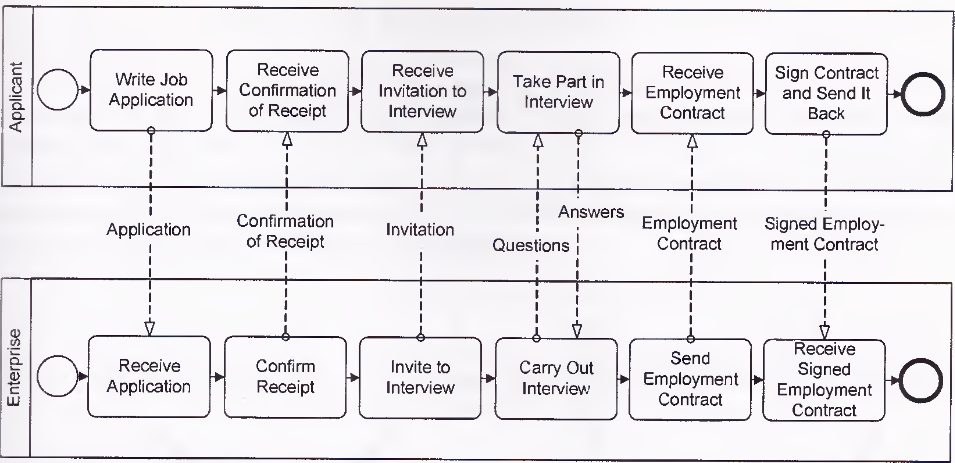
\includegraphics[width=11cm]{./imagenes/diagrama_colaboracion.png}
    \caption{Ejemplo de diagrama de colaboraci�n}
    \label{fig:diagrama_colaboracion}
    \textbf{Fuente:}  \cite{bpmn2}
  \end{center}
\end{figure}


Por ejemplo, la actividad ``Recibir solicitud'' recibe un mensaje de la actividad ``Redactar solicitud de empleo'', por lo cual esta actividad (recibir solicitud) no puede iniciar si el aspirante no env�a su solicitud. Esto significa que los mensajes deben ser respetados y una actividad no puede realizarse si le falta alg�n mensaje de entrada.

Sin embargo, en estos casos solo se conoce el proceso que sigue la empresa, por lo que es com�n representar a las partes externas como una caja negra (figura \ref{fig:diagrama_colaboracion_caja_negra}).

\begin{figure}[!htb]
  \begin{center}
    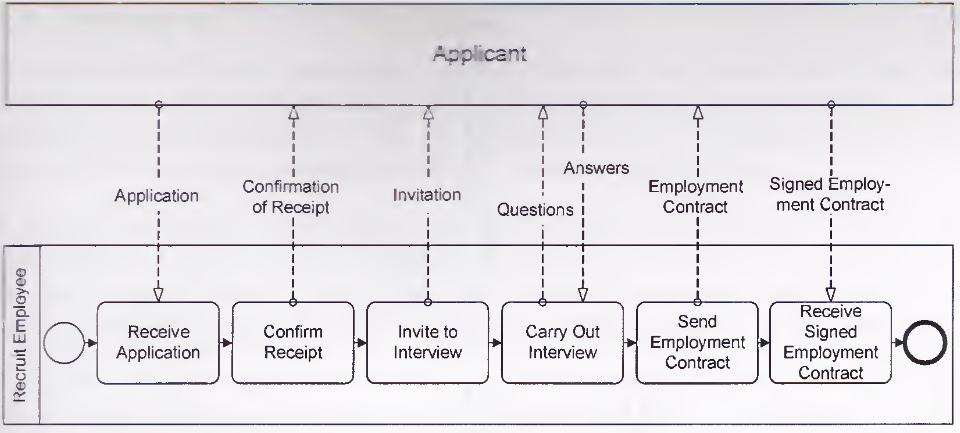
\includegraphics[width=11cm]{./imagenes/diagrama_colaboracion_caja_negra.png}
    \caption{Ejemplo de diagrama de colaboraci�n con caja negra}
    \label{fig:diagrama_colaboracion_caja_negra}
    \textbf{Fuente:}  \cite{bpmn2}
  \end{center}
\end{figure}
